\section{Experimental results}\sloppy
\label{sec:exp}

  % Here you evaluate your work using experiments. You start again with a
  % very short summary of the section. The typical structure follows.
  %
  % \mypar{Experimental setup} Specify the platform (processor, frequency, maybe OS, maybe cache sizes)
  % as well as the compiler, version, and flags used. If your work is about performance, 
  % I strongly recommend that you play with optimization flags and consider also icc for additional potential speedup.
  %
  % Then explain what kind of benchmarks you ran. The idea is to give enough information so the experiments are reproducible by somebody else on his or her code.
  % For sorting you would talk about the input sizes. For a tool that performs NUMA optimization, you would specify the programs you ran.

\mypar{Experimental setup}
Benchmarks were run on two distinct setups: a node of ETH's Euler cluster, a convential x86 multicore platform, and on ETH's Einstein machine with ssh-access to a Knight's Corner Intel Xeon Phi coprocessor. An Euler node consists of two Intel Xeon E5-2697v2 processors for a total of 24 x86 cores in a dual-socket NUMA setup. The x86 benchmark code was compiled with GCC 4.9.2 with OpenMP 4.0, while the Xeon Phi host code was compiled with GCC 4.8.2. Both setups used precompiled TBB 4.4 for
parallelization. The Xeon
Phi setup additionally uses the MPI library from Intel Parallel Studio XE 2016 when communicating with the Xeon Phi on both host and coprocessor, and the MIC code (\texttt{-mmic}) is compiled using ICC 15.0.0. All code was compiled with \texttt{-std=c++11}, \texttt{-O3} and \texttt{-march=native} for both GCC and ICC. 

\mypar{Data set}


  % \mypar{Results}
  % Next divide the experiments into classes, one paragraph for each. In each class of experiments you typically pursue one questions that then is answered by a suitable plot or plots. For example, first you may want to investigate the performance behavior with changing input size, then how your code compares to external benchmarks.
  %
  % For some tips on benchmarking including how to create a decent viewgraph see pages 22--27 in \cite{Pueschel:10}.
  %
  % {\bf Comments:}
  % \begin{itemize}
  %   \item Create very readable, attractive plots (do 1 column, not 2 column plots
  %     for this report) with readable font size. However, the font size should also not be too large; typically it is smaller than the text font size.
  %     An example is in Fig.~\ref{fftperf} (of course you can have a different style).
  %   \item Every plot answers a question. You state this question and extract the
  %     answer from the plot in its discussion.
  %   \item Every plot should be referenced and discussed.
  % \end{itemize}
  %
  % \begin{figure}\centering
  %   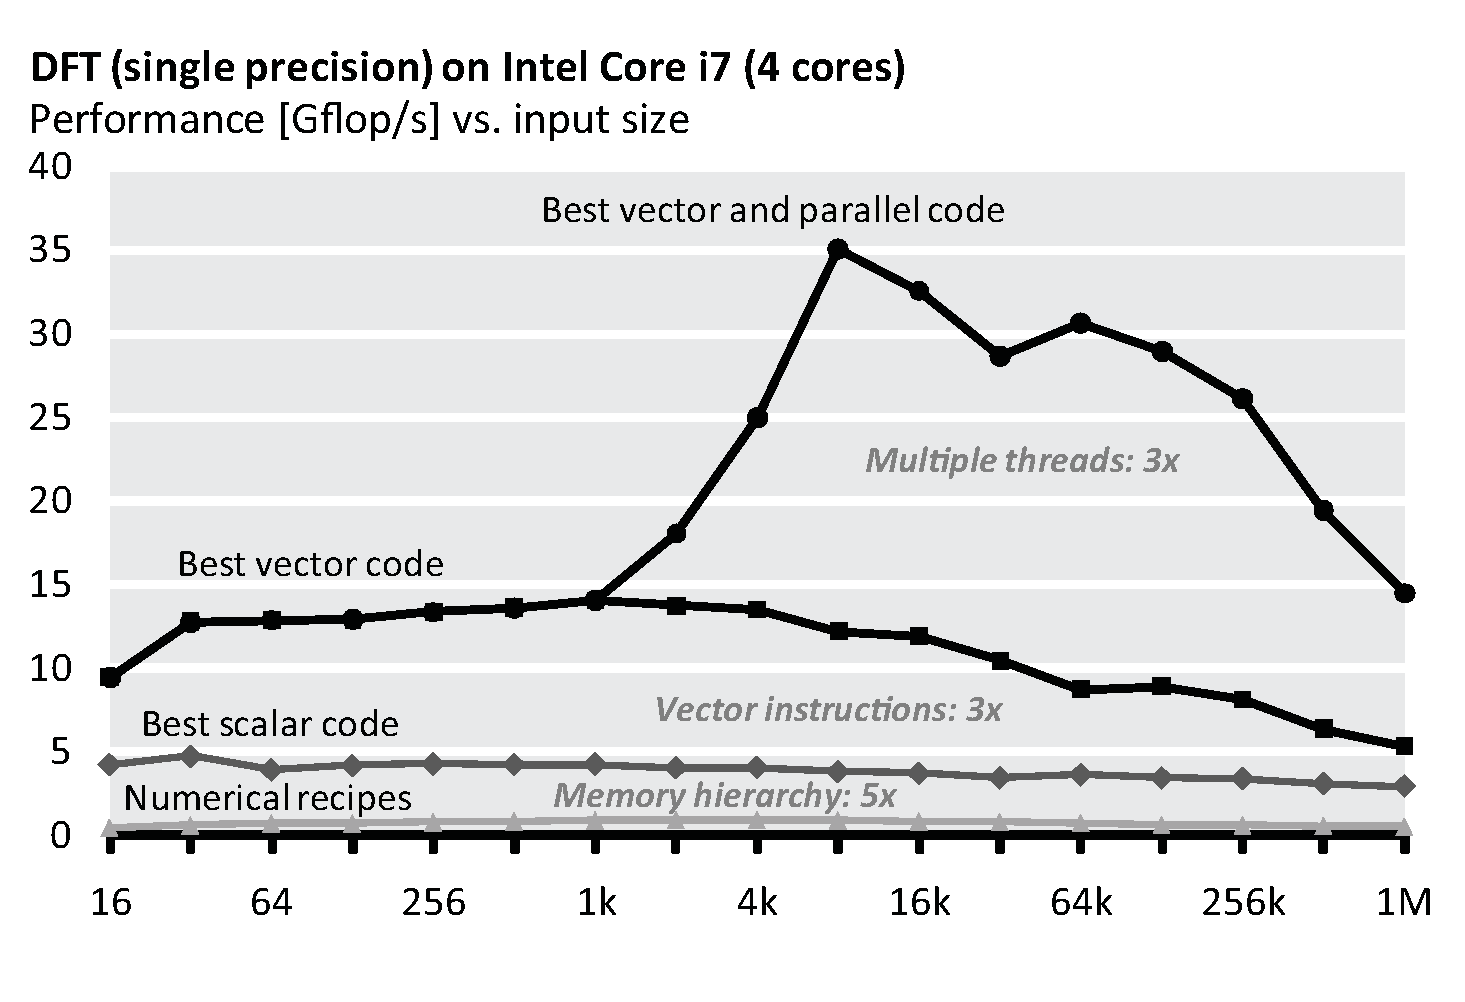
\includegraphics[scale=0.33]{./03_results/figs/dft-performance.eps}
  %   \caption{Performance of four single precision implementations of the
  %   discrete Fourier transform. The operations count is roughly the
  %   same. The labels in this plot are maybe a little bit too small.\label{fftperf}}
  % \end{figure}

\mypar{Build performance.} Parallel build of the randomized kd-trees is done on the TexMe 

  % mainfile: ./../report.tex
